\chapter{Desarrollo de la Evaluación Automática}\label{chapter: Automatic-Eval}

En este capítulo se presenta el desarrollo de los métodos que se ejecutan en la evaluación automática, y la incorporación de la cinta computacional al grafo de evaluación. 

En la sección \ref{3:VRP-eval} se presentan los diferentes problemas de enrutamiento de vehículos que se pueden presentar para evaluar. En la sección \ref{3:init-Solution} se presenta cómo se realiza la evaluación de la solución inicial. En la sección \ref{3:neighbor-solutions} se presenta cómo se modifica este grafo y cómo se realiza la evaluación eficiente de las soluciones vecinas del VRP. En la sección \ref{3:VRP-limits} se presentan algunas variantes que no pueden aplicar la evaluación automática solamente con el grafo de evaluación. En la sección \ref{3:tape-development} se presenta la incorporación de la cinta al grafo de evaluación.

\section{Tipos de VRP a evaluar}\label{3:VRP-eval}
En esta sección se presentan los diferentes tipos de variantes de VRP que pueden presentarse en cualquier escenario.

Existen muchas variantes de VRP y es difícil garantizar que para cualquiera de ellos solo una parte de ese problema se afectará al aplicarle un criterio. Existen tres posibilidades para la evaluación automática de un sistema de enrutamiento de vehículos.

\bf{Definición 1:} \it Llamaremos VRP con clientes independientes a aquellos problemas donde las variables de evaluación o restricción de un cliente (ya sea tiempo, combustible, dinero, distancia, capacidad, etc) no afectan a otro cliente. En ese caso, los clientes son independientes. 

\rm{Este tipo de problemas tiene características especiales en el grafo de evaluación. Cada nodo auxiliar provee directamente al sumador parcial de la ruta y no a otro nodo auxiliar. Se puede notar en la figura \ref{fig:ICVRP}.}

\begin{figure}[htb]
	\centering
	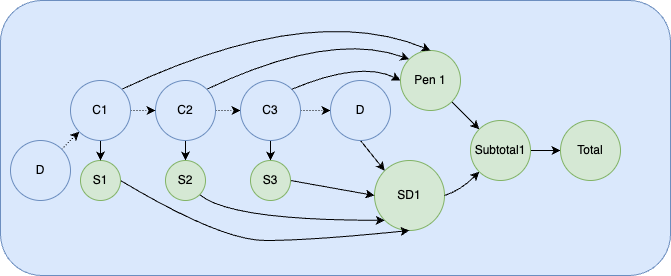
\includegraphics[width=0.7\linewidth]{Graphics/ICVRP}
	\caption{Grafo de evaluación de un VRP con variables independientes.} 
	\label{fig:ICVRP}
\end{figure}

Sobre ese tipo de problemas se tiene el siguiente teorema:
\\\\
\bf{Teorema 1:} \it{En un VRP con clientes independientes, al transformarse un cliente en una ruta solo será necesario reevaluar ese cliente que tributará a la variable de penalización y de suma parcial de la ruta y a la variable del valor final.} 
\\\\
\rm No será necesario reevaluar ningún otro cliente. Al ser independiente del resto no afectará en nada un cambio en su evaluación. Si se agrega o se elimina un cliente, por ejemplo, la evaluación de cada cliente será exactamente igual, no se necesita computar nuevamente la ruta completa. Lo mismo ocurre con rutas disjuntas a la modificada.
\\\\
\bf{Definición 2:} \it Llamaremos VRP con rutas disjuntas a los problemas donde las rutas son independientes. Es decir, las características de los clientes de una ruta no interfieren o modifican a las de la otra ruta.

\rm{Este tipo de problemas es el más común. La mayoría de los VRP se pueden modificar y convertir a este tipo de problemas. La figura \ref{fig:vrp-changeClient} muestra un grafo de evaluación de este tipo.}

\bf{Teorema 2:} \it En los VRP con rutas disjuntas, al ser modificada una de sus rutas será necesario reevaluar, solamente, la ruta modificada, la evaluación de las rutas restantes será la misma después de la modificación del sistema.

\rm Como las demás rutas no se ven afectadas, entonces, por definición, no será necesario comprobar un cambio en su evaluación anterior, el valor y los componentes seguirán siendo los mismos luego que se modifique dicha ruta.

En estos problemas hay dos casos posibles. En primer lugar, la modificación de un cliente afecta la ruta a partir de él hasta cierto cliente o hasta el final de la ruta, es decir, afecta una subruta. Se muestra este caso en la figura \ref{fig:Subway} donde se afecta desde el cliente 1 hasta el cliente 3, sin embargo, no es necesario volver a evaluar el cliente 4, ya que no se ve afectado.

\begin{figure}[htb]
	\centering
	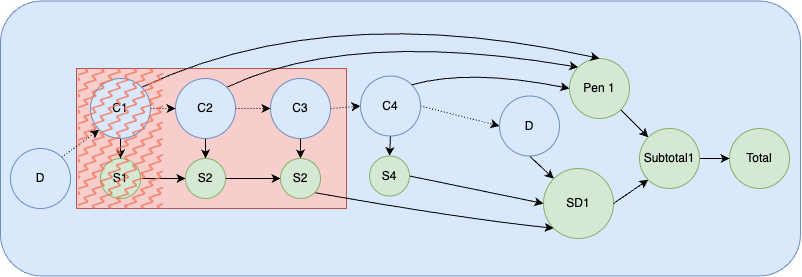
\includegraphics[width=0.7\linewidth]{Graphics/Subway}
	\caption{Grafo de evaluación de un VRP con rutas disjuntas. Caso donde solo se afecta una subruta.} 
	\label{fig:Subway}
\end{figure}


El segundo caso ocurre cuando la modificación de un cliente afecta a toda la ruta, y es necesario reevaluarla completa. Por ejemplo cuando cambia el depósito inicial, o las características de un cliente afectan al cliente anterior. En este caso, se debe reevaluar la ruta completa ya que se afectan todos los clientes. Se muestra este caso en la figura \ref{fig:vrp-changeClient} donde se afecta desde el cliente 1 hasta el cliente 4.

Los VRP con clientes independientes son un subconjunto del primer caso. Y estos, a su vez, son un subconjunto del segundo caso.

\bf{Definición 3:} \it Llamaremos VRP con rutas mezcladas a los problemas donde las rutas no son todas independientes. 

\rm En este caso al trasformarse una ruta que no es disjunta se debe reevaluar todo el sistema teniendo un costo igual a la primera evaluación. 

\section{Evaluación de la solución inicial}\label{3:init-Solution}
En el capítulo \ref{chapter: VRP} se mostró cómo se obtenía el grafo de evaluación a partir de la solución inicial. En esta sección se describe cómo se alcanza la evaluación de esa solución inicial.

En cada nodo principal del grafo de evaluación que representa una entidad del problema se puede acceder a la  información del problema que es relevante a esa entidad \cite{JJ}. Es decir, cada nodo que represente a algún cliente contiene la distancia hacia los demás clientes, las demandas y otra información que sea importante para el cliente. Lo mismo ocurre con el resto de los nodos principales.

A los nodos intermedios creados en el proceso de evaluación se le asocia la operación a realizar sobre las demandas de los clientes y dos métodos, uno para evaluar, y otro para desevaluar, que deshace la evaluación. 

Por ejemplo, si la operación es incrementar la demanda de la ruta, entonces el método evaluar del nodo intermedio asociado a cada cliente suma la demanda del cliente y el valor obtenido del nodo intermedio anterior. El método desevaluar se utiliza para cancelar el método de evaluación de un nodo intermedio.

Al final de cada ruta, el nodo intermedio asociado al último cliente contiene el valor de la evaluación de toda la ruta.

Además de esos nodos intermedios, se crea un nodo penaliza que guarde en cuánto se incumple la demanda de cada cliente en la solución evaluada. En otro nodo intermedio se guarda la evaluación de la ruta una vez penalizada. El valor final de la evaluación de la solución se obtiene a partir de las evaluaciones penalizadas de cada ruta.

Una vez obtenida la evaluación de la solución inicial queda construido totalmente el grafo de evaluación que permitirá evaluar automáticamente soluciones vecinas. Esto se muestra en la siguiente sección.

\section{Obtención y evaluación de las soluciones vecinas} \label{3:neighbor-solutions}

Si se realizan transformaciones a la solución inicial pueden obtenerse soluciones vecinas que se evalúan automáticamente utilizando el grafo de evaluación. En esta sección se presenta cómo se evalúan estas soluciones y una propuesta para que funcione en cualquier VRP.

En el capítulo \ref{chapter: VRP} se mostró cómo se modifica el grafo de evaluación al aplicar una operación sobre la solución inicial. Cada operación es un método que transforma el grafo de evaluación y evalúa o desevalúa los nodos intermedios afectados por la modificación.

Por ejemplo, en la figura \ref{fig:vrp-deleteClient} se aplica la transformación \textbf{eliminar cliente}. Este es un método que recibe las coordenadas del cliente, es decir, el índice de la ruta en la que se encuentra y su posición en la ruta. El nodo intermedio asociado a ese cliente se desevalúa y se elimina, se conecta el nodo intermedio anterior a él con el nodo intermedio siguiente y se evalúan los nodos intermedios afectados. En el ejemplo de la figura, se deben evaluar todos los nodos intermedios siguientes al nodo eliminado.

En \cite{JJ} el autor propone almacenar el nodo extraido en una lista de clientes extraidos.

Los métodos que realizan las operaciones de modificación de una solución son comunes para cualquier VRP que se desee resolver, debido a que los métodos de evaluación y desevaluación reciben la operación a partir del nodo intermedio y, las demandas, a partir de los clientes. 

Un criterio de vecindad es un conjunto de operaciones que modifican la solución inicial, como se plantea en el Capítulo \ref{chapter: VRP}. Al aplicar los métodos de cada una de las operaciones que componen el criterio de vecindad que se utilice, se obtiene la evaluación de la nueva solución. Solamente se reevalúan los nodos del grafo que se modificaron por la aplicación de dichas operaciones. Esta evaluación automática se realiza sin repetir cálculo innecesario.

Este proceso de evaluación automática, como se ha presentado hasta aquí, no funciona para todas las variantes de VRP. En la siguiente sección se presentan algunas de estas variantes.

\section{Limitaciones de algunos VRP}\label{3:VRP-limits}

En esta sección se presentan algunas variantes que no pueden utilizar solamente el grafo de evaluación en la evaluación de sus soluciones vecinas.

En algunos problemas de enrutamiento de vehículos como, por ejemplo, el Problema de Enrutamiento de Vehículos con Entregas y Recogidas Simultáneas o el Problema de Enrutamiento de Vehículos con Ventanas de Tiempo, es necesario evaluar otros nodos del grafo de evaluación que no fueron modificados en la aplicación del criterio de vecindad.

En el Problema de Enrutamiento de Vehículos con Entregas y Recogidas Simultáneas, cada cliente recibe y devuelve una cierta cantidad de producto al mismo tiempo. En esta variante, cada cliente es visitado una única vez, lo que da nombre a este VRP. Esto puede llevar a la violación de la restricción de capacidad, ya que la cantidad total de producto que mantiene el vehículo en cada entrega y recogida puede exceder su capacidad, debido a la recogida de productos mientras se atiende a un cliente durante el recorrido. Por tanto, es necesario penalizar el exceso de carga al visitar cada cliente de la ruta, durante el recorrido y no al final de este.

Si el proceso de penalización se realizara al final de ruta, como ocurre en CVRP (VRP con restricción de capacidad), se puede transformar la solución y reevaluarse hasta el final sin problemas. Sin embargo, si ocurre como en el caso anterior, que la penalización ocurre durante el recorrido, al realizar una modificación de la solución debe verificarse si el cliente modificado participó o no en la penalización de la ruta.

Lo mismo ocurre en el Problema de Enrutamiento de Vehículos con Ventanas de Tiempo, en el que cada cliente tiene un rango de tiempo para satisfacer su demanda. La penalización ocurre cuando el vehículo no llega en ese rango de tiempo que el cliente presenta. Como esta penalización ocurre durante el recorrido y no al final de la ruta, se debe poder verificar en la modificación de la solución, si el cliente afectó o no la variable penalizar.

En la siguiente sección se muestra la propuesta de solución a esta limitante.

\section{Cinta computacional}\label{3:tape-development}

En esta sección se plantean la propuesta de solución que resuelve las limitaciones de algunos VRP frente a la evaluación automática.

El problema que se presenta se basa en la modificación de las variables que se utilizan en la evaluación final del recorrido o ruta. Tal es el caso de la penalización.

Para resolver el problema, se propone implementar la cinta que utiliza la diferenciación automática, que se desarrolla en el capítulo \ref{chapter: AD}. Esta cinta regula las operaciones de modificación sobre la solución inicial. 

En primer lugar, se debe definir cada operación que forma parte de los criterios de vecindad que se aplican a la solución para obtener soluciones vecinas. Al obtener las operaciones y la posición donde se aplicará, se devuelve la parte de la solución que se afecta por esa modificación.

\begin{figure}[htb]
	\centering
	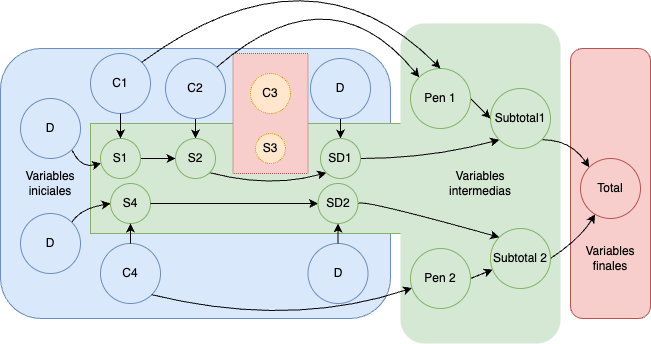
\includegraphics[width=0.7\linewidth]{Graphics/DeleteClient}
	\caption{Grafo de evaluación transformado al eliminar el cliente 3.}
	\label{fig:lisp-deleteClient}
\end{figure}

Si se toma el ejemplo representado en la figura \ref{fig:lisp-deleteClient}, donde se elimina al cliente 3 de la ruta 1 la operación es \textit{eliminar cliente}. A ese método se le pasan los argumentos \textit{ruta: 1} y \textit{posición: 3}. 

A partir de la operación eliminar cliente en la cinta, se verifica la parte de la solución que se modifica y se debe reevaluar. En el caso del ejemplo, se debe reevaluar a partir del cliente anterior hasta el final de la ruta. Para saber si el cliente eliminado afectó la variable penalización este nodo debe ser diferente a los demás nodos intermedios, guardando el valor de penalización de todos los clientes a los que no se les satisfizo la demanda y, por tanto, aumentaron la penalización de la ruta. Por tanto, cuando se elimine al cliente \textit{$C_{3}$} se reevaluará desde el nodo intermedio asociado al nodo del cliente 2 hasta el nodo de salida final, teniendo en cuenta que del nodo penalización se eliminará cualquier penalidad asociada al cliente eliminado.

En el caso de la figura \ref{fig:lisp-insertClient}, donde se inserta el cliente eliminado en la ruta 2, se realiza el mismo proceso de la ruta 1 en la ruta 2. 

\begin{figure}[htb]
	\centering
	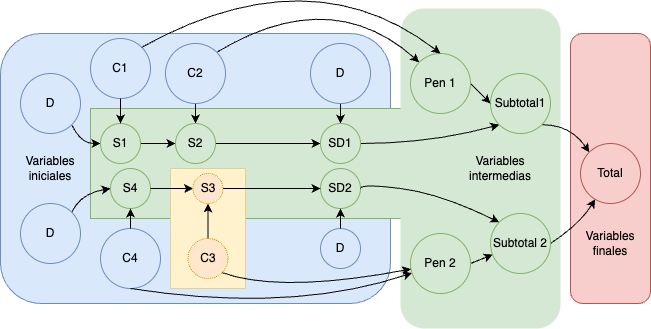
\includegraphics[width=0.7\linewidth]{Graphics/ChangeClient}
	\caption{Grafo de evaluación transformado al eliminar el cliente 3.}
	\label{fig:lisp-insertClient}
\end{figure}

Como la operación es de insertar, entonces, además de evaluar a partir de él, se debe actualizar la variable penalización, en caso de que no se cumpla con la demanda del cliente insertado.

Todas las variables que se modifican en el recorrido en cualquier VRP deben guardar todos los clientes que modifican su valor, como \textbf{penalización} en este caso. Esto hace menos eficiente el algoritmo de evaluación de la solución. En cada variable de ese tipo debe evaluarse el valor de la variable al final de la ruta.

La cinta de evaluación para el ejemplo de la figura \ref{fig:lisp-deleteClient} quedaría de la siguiente manera:

\begin{itemize}
    \item Eliminar cliente (1,3)
    \item Reevaluar (1, 2)
\end{itemize}

Los parámetros de Eliminar cliente son la ruta y la posición del cliente en la ruta. Los parámetros de reevaluar son la ruta y la posición desde donde se debe evaluar.

La cinta de evaluación para el ejemplo de la figura \ref{fig:lisp-insertClient} quedaría de la siguiente manera:

\begin{itemize}
    \item Insertar cliente (2,2)
    \item Reevaluar (2,1)
\end{itemize}

Una solución alternativa es evaluar toda la ruta cuando esta contenga alguna variable que se modifica en el recorrido, como \textbf{penalización}. El cliente que modifique alguna variable durante el recorrido de la ruta debe guardarse en la cinta para verificarse en caso de una modificación para encontrar soluciones vecinas.

La cinta de evaluación para el ejemplo de la figura \ref{fig:lisp-deleteClient} con esta propuesta se muestra en la figura \ref{tape-delete-client}

\begin{figure}[h!]
    \begin{verbatim} 
    clientes_penalizados 
    Eliminar cliente (1,3)
    por cada cliente_i en clientes_penalizados:
             si cliente_i en ruta 1 y posición cliente_i <
                                            posición cliente 3
                Evaluar ruta 1
                terminar
    Reevaluar (1,3)
    \end{verbatim}
    \caption{Cinta de evaluación para el ejemplo \ref{fig:lisp-deleteClient}.\label{tape-delete-client}}
  \end{figure}


La cinta de evaluación para el ejemplo de la figura \ref{fig:lisp-insertClient} se muestra en la figura \ref{tape-insert-client}:

\begin{figure}[h!]
    \begin{verbatim} 
    cliente_i
    Insertar cliente (2,2)
    por cada cliente_i en clientes_penalizados:
             si cliente_i en ruta 2 y posición cliente_i <
                                            posición cliente 2
                Evaluar ruta 2
                terminar
    Reevaluar (2,2)
\end{verbatim}
\caption{Cinta de evaluación para el ejemplo \ref{fig:lisp-insertClient}.\label{tape-insert-client}}
\end{figure}

Al utilizar un criterio de vecindad, varias operaciones se desarrollan en la cinta de evaluación. En la figura \ref{tape-move-client} se muestra el criterio \textit{cambiar un cliente de posición}.

\begin{figure}[h!]
    \begin{verbatim} 
    clientes_penalizados 
    Eliminar cliente (1,3)
    por cada cliente_i en clientes_penalizados:
             si cliente_i en ruta 1 y posición cliente_i <
                                            posición cliente 3
                                                        
                Evaluar ruta 1
                terminar
    Reevaluar (1,3)
    Insertar cliente (2,2)
    por cada cliente_i en clientes_penalizados:
             si cliente_i en ruta 2 y posición cliente_i < 
                                           posición cliente 2
                Evaluar ruta 2
                terminar
    Reevaluar (2,2)
    \end{verbatim}
    \caption{Cinta de evaluación usando el criterio \textit{cambiar un cliente de posición}.\label{tape-move-client}}
  \end{figure}

Esta propuesta realiza más cálculos que las modificaciones que se realizan en la ruta. Pero garantiza que se evalúen los vecinos de cualquier problema de enrutamiento de vehículos. 

En este capítulo se explicaron los métodos que se ejecutan en la evaluación automática de las soluciones vecinas, y la incorporación de una cinta computacional al grafo de evaluación para que sea posible usar esta estrategia en cualquier problema de enrutamiento de vehículos. En el siguiente capítulo se explica cómo se utiliza la evaluación automática en algunas variantes en las que no era posible utilizarse.

% Chapter 4 Resultados

% Conclusiones, recomendaciones y bibliografía



























